\documentclass[12pt, final]{article}
\usepackage[margin= 0.75in]{geometry}
\usepackage{amsfonts}
\usepackage{amsthm}
\usepackage{amsmath}
\usepackage{mathabx}
\usepackage{ulem}
\usepackage{enumerate}
\usepackage{float}
\usepackage{graphicx}
\graphicspath{{../Code/PLOTS/}}
\usepackage{color}
\usepackage{subfigure}
\usepackage{commath}
\usepackage[font = scriptsize]{caption}

\begin{document}

\newcommand{\Pois}{\text{Pois}}

\newtheorem{prop}{Proposition}


\title{Think of a title later}
\author{Ansel Blumers and Ankan Ganguly}
\maketitle

\begin{abstract}
Abstract goes here.
\end{abstract}

\newpage

\tableofcontents

\newpage

\section{Introduction}

Write an introduction here.

\section{Methods}

In this paper, we used the simulated Integrate and Burst model introduced in \cite{Fiete}. We then implemented STDP learning and Hebbian learning.

\subsection{Integrate and Burst Model}

Our integrate and burst model is an implementation of equations described in \cite{Fiete}. We provide a detailed description of those equations here, with more attention paid to the intuition behind these equations. There are \(N\) neurons connected in an all-to-all environment. Each neuron \(i\) bursts when its membrane potential, \(V_i\), hits the threshold \(V_\theta\). We assume that every neuron bursts for \(T_{burst}\) time. While bursting, each neuron fires four times uniformly over the burst interval before resetting to \(V_{reset}\).

When a neuron is not bursting, its potential is governed by a typical conductance based leaky integrate and fire model with built-in inhibition:

\begin{equation}
\tau_V \od{V_i}{t} = -g^L(V - V^L) - g^E_i(V - V^E) - g^I_i(V - V^I)
\label{Potential}
\end{equation}

The leak conductance, \(g^L\), is assumed to be a homogeneous constant input, as is the leak potential \(V^L\). Notice that in the absence of excitatory or inhibitory conductance, neuron \(i\) will tend to \(V^L\). Therefore we can say that the leak potential is also equal to the rest potential.

The excitation potential, \(V^E\), and the inhibition potential, \(V^I\), act as upper and lower bounds on untethered \textcolor{red}{(What was the word for IF potential plots without a firing threshold?)} potential respectively. 

The excitation conductance, \(g^L\), is defined by the activity in neighboring neurons as well by external random stimulation:

\[g^L = Ws + W_0b\]

Where \(W_{ij}\) is the strength of the synapse from neuron \(j\) to neuron \(i\), \(W_0\) is the conductance strength of external synapses and \(b\) is a Poisson random variable with frequency \(r_{in}\). \(r_{in}\) was an input parameter. In \cite{Fiete} \(r_{in}\) was constant, but we chose to assign \(r_{in}\) a high value and anneal it to jump-start neural activity. \(s_i\) is the activation of neuron \(i\). It is incremented each time neuron \(i\) fires, and it decays by

\[\od{s}{t} = -\tau s\]

The inhibitory conductance, \(g^I\), is defined as the sum of the adaptation inhibition, \(g^I_{ada}\), and the global inhibition, \(g^I_{glob}\). The adaptation inhibition is the internal inhibition generated by activation of a neuron. It is defined by the same equations as \(s_i\), but with a constant multiplier \(A_a\) and a slower time-constant \(\tau_{ada}\).

\subsection{Learning}

The purpose of this paper is to replicate and test some of the claims made in \cite{Fiete}. One of the claims made is that the model used by \cite{Fiete} demonstrates how STDP can contribute to the synchronous regular synfiring chains exhibited in Zebra Finch \textcolor{red}{(Where? Maybe cite second paper here?)}. We implemented STDP, but we also implemented a pure Hebbian learning rule to demonstrate that STDP learning is not necessary for the model to exhibit synchronous regular firing chains.

\subsubsection{STDP Learning}

We followed \cite{Fiete} precisely in our implementation of STDP learning. Define

\[K(t) = 
\begin{cases}
e^{-t/\tau_{STDP}} &\text{ if } t > 0\\
-e^{-t/\tau{STDP}} &\text{ if } t < 0\\
0 &\text{ otherwise}
\end{cases}
\]

as the STDP kernel. For every pair of neurons \(i,j\), let \(t_i < t_j\) be two times when \(i\) and \(j\) fired respectively. Then According to STDP, the weight matrix element \(W_{ij}\) should increase proportional to \(K(t_j - t_i)\). Notice that the change in \(W\) according to STDP is approximately anti-symmetric. \cite{Fiete} strengthened the nonlinearity of STDP by making STDP growth of a synapse proportional to the strength of that synapse (with an added factor so 0 weight synapses could grow). In particular, the paper defined:

\begin{equation}
\Delta^{STDP}_{ij}(t) = \left(\frac{W_{ij}(t-1)}{w_{max}} + 0.001\right)*\left(x_i(t)K(0)x_j(t) + \sum_{\tau = 0}^t  [x_i(t)K(\tau)x_j(t -\tau) - x_i(t - \tau)K(\tau)x_j(t)]\right)
\label{STDP}
\end{equation}

Where \(x_i(t)\) is a binary variable taking the value 1 if neuron \(i\) fired at time \(t\). So, at each time \(t\), \(\Delta^{STDP}(t)\) is proportional to the change in \(W\) with respect to STDP. Our implementation assumed \(K(t) \approx 0\) for \(t > 4\)ms.

However, the key innovation of this paper was to introduce a secondary source of competition. If the total strength of all synapses into or out of a given neuron exceed a soft limit \(W_{max}\) after STDP learning, then all such synapses experience long-term depression (LTD) proportional to the amount by which the soft limit is exceeded:

\begin{equation}
\theta^{col}_i =  \left[\sum_{j=1}^N (W_{ij} + \eta\Delta^{STDP}_{ij}) - W_{max}\right]^+
\label{hLTP}
\end{equation}

\(\theta^{col}\) denotes the amount by which the soft limit has been exceeded \footnote{Our implementation was a little different and \cite{Fiete} defined \(\theta^{col}\) differently, however this is the correct way to define \(\theta^{col}\). See the results and discussion for more details.}. Define \(\theta^{row}\) similarly. Then,

\begin{equation}
\od{W_{ij}}{t} = \eta\Delta^{STDP}_{ij} - \epsilon(\theta^{col}_i + \theta^{row}_j)
\label{Learning}
\end{equation}

This updates weights according to STDP along with a penalty if the soft limit is exceeded. Finally, to ensure that STDP never diverges, we implement a hard limit. If any element \(W_{ij}(t) > w_{max}\), where \(w_{max}\) is a constant parameter, we manually set \(W_{ij}(t)\) to \(w_{max}\). 

\subsubsection{Hebbian Learning}

Hebbian plasticity is a general family of learning rules which strengthen synapses between neurons which fire with high correlation. Hebbian learning rules are generally considered incomplete because while they explain how synapses are strengthened, they do not explain how synapses might be weakened. 

One way to complete the Hebbian learning rule is with STDP. In STDP learning, highly correlated neurons experience a large change in synaptic strength, but the direction of the change (increase or decrease) depends on the relative timing of firing between the synapses.

However, the soft and hard limits imposed by the model also provide a way for synapse strength to decrease, so it should be possible to implement this model using Hebbian plasticity. To do this, we ran the exact same learning algorithm as implemented for STDP, but we modified the kernel to be

\[K(t) = 
\begin{cases}
e^{-t/\tau_{Heb}} &\text{ if } t > 0\\
0 &\text{ otherwise}
\end{cases}
\]

With this new kernel, 

\begin{equation}
\Delta^{Heb}_{ij}(t) = \left(\frac{W_{ij}(t-1)}{w_{max}} + 0.001\right)*\left(x_i(t)K(0)x_j(t) + \sum_{\tau = 0}^t  x_i(t)K(\tau)x_j(t -\tau)\right)
\label{Heb}
\end{equation}

gives us a Hebbian learning rule. We implemented the soft and hard synaptic weight limits as in STDP learning.

\subsection{Parameter Choices}

Our implementation of the Integrate and Burst neuron network with STDP learning matched that used in \cite{Fiete} in many cases. However a few parameters were chosen differently. The table below provides a list of parameters we used:

\begin{center}
\begin{tabular}{|c|c|p{0.5cm}|c|c|p{0.5 cm}|c|c|}
\cline{1-2}\cline{4-5}\cline{7-8}
Parameters & Values & & Parameters & Values& & Parameters& Values\\

\cline{1-2}\cline{4-5}\cline{7-8}
\(dt\) & \(2 \times 10^{-5}\)s& & \(\tau_V\) & 0.01 F/m\(^2\)& &\(V^L\) & -0.06V\\

\cline{1-2}\cline{4-5}\cline{7-8}
\(V^E\) & 0V& & \(V^I\) & -0.07V& & \(W_0\) & 5S/m\(^2\)\\

\cline{1-2}\cline{4-5}\cline{7-8}
\(V_{\theta}\) & -0.05V & & \(V_{reset}\) & -0.055V & & \(T_{burst}\) & 0.006s\\

\cline{1-2}\cline{4-5}\cline{7-8}
\(\tau\) & 0.004s & & \(r_{in}^{start}\) & 10000Hz & & \(r_{in}^{min}\) & 4000Hz, 6000Hz\\

\cline{1-2}\cline{4-5}\cline{7-8}
\(N\) & 50 & & \(w_{max}\) & 0.14 & & \(W_{max}\) & 0.14\\

\cline{1-2}\cline{4-5}\cline{7-8}
\(\eta\) & varies & & \(\epsilon\) & varies & & \(A_g\) & 4\\

\cline{1-2}\cline{4-5}\cline{7-8}
\(A_a\) & 9 & & \(\tau_{STDP}= \tau_{Heb}\) & 0.02s & & \(\tau_{ada}\) & 0.015s\\
\end{tabular}
\end{center}

\section{Results}

Introduce the big idea and what we got.

\subsection{Parameter Tuning}

\begin{itemize}
\item 4000 Hz doesn't work! (Burst Plot)

\item Mention annealing and our choice of \(r_{in}, \eta\) and \(\epsilon\). Name the two data sets we refer to for the remainder of the paper. (Scatter Error Function)

\item Setting \(w_{max}\). (Burst History)
\end{itemize}

\subsection{Convergence and Stability}

\begin{itemize}
\item Demonstrate the stability of our IB model by showing the firing rate plot and how it splits according to \(r_{in}\).

\begin{figure}[H]
\centering
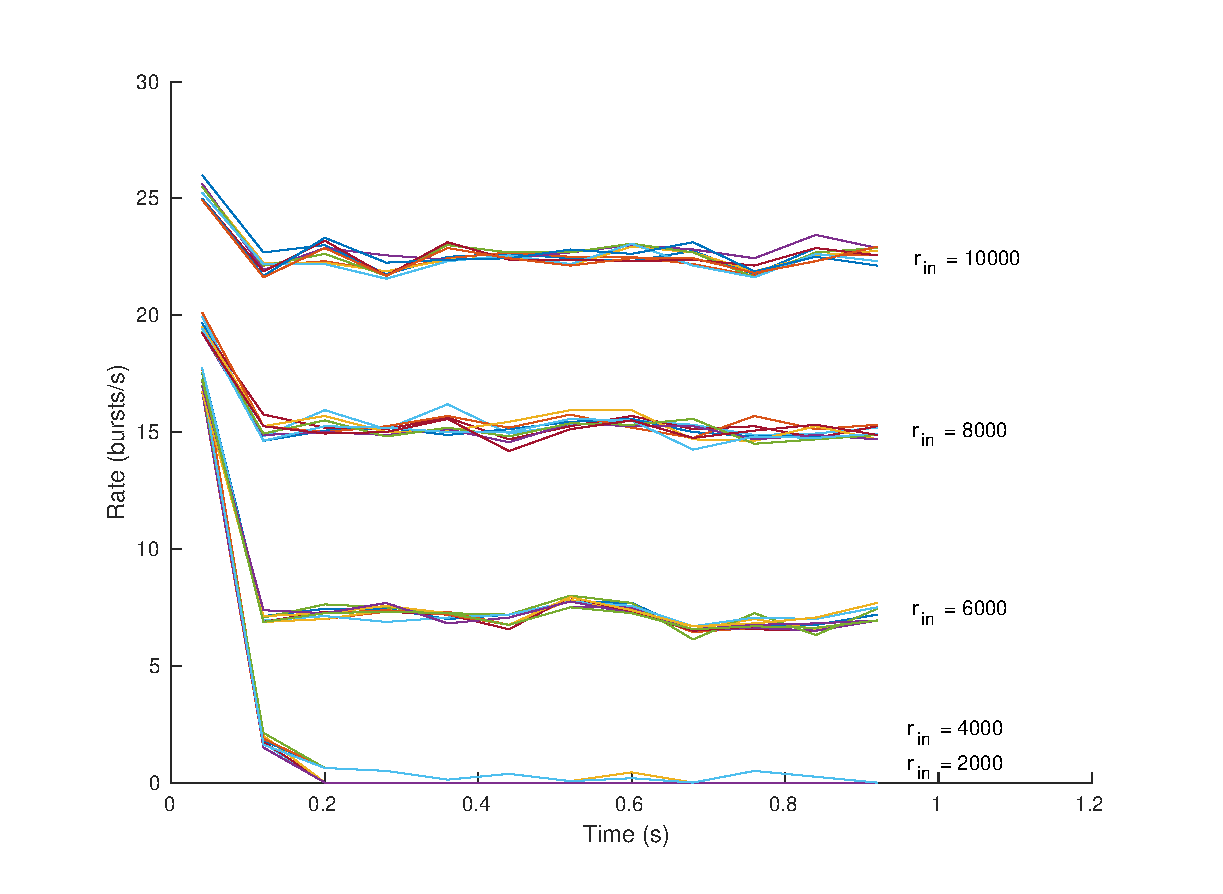
\includegraphics[scale = 0.4]{Firing_Rate_Binsize_80ms.eps}
\label{FR}
\caption{Caption will go here}
\end{figure}

\item Plot Weight and \(WW^T\) for 4000 and 6000 Hz to show some level of convergence.

\item Plot error function over time from normal and from permutation matrix

\item Describe why the error function converges away from 0.
\end{itemize}

\subsection{Hebbian Learning versus STDP}

\begin{itemize}
\item Introduce the idea of the refutation. 
\item Give a theoretical description why the type of learning should be relatively unimportant.
\item Compare plots (\(WW^T\), Error vs Time, Burst History).
\end{itemize}

\section{Discussion}

Further improvements that could be made to our model and where this research could be taken.

\section{Summary}

Quick summary of our results and everything.



\bibliographystyle{plain}
\bibliography{Songbird_paper}

\end{document}